\section{Related Work}
\label{related_work}
There are three different categories of cache organizations:
\begin{itemize}
	\item \textbf{Direct Mapped}: every memory block brought to the cache has exactly one place. It's fast but potentially resulting in poor utilization of the total cache.
	
	\item \textbf{Fully Associative Mapped}: every memory block can be placed in any available cache line. It has high implementation overhead but better cache utilization.
	
	\item \textbf{Set Associative Mapped}: every memory block can be placed in a particular set in the cache. 
\end{itemize}

Generally speaking, we have two hashing methods categories: data-independent and data-dependent. Data-independent hashing methods usually generate a set of hash functions using randomization (without using any training data). In contrast,  data-dependent hashing methods usually are using unsupervised, supervised or semi-supervised learning techniques to generate the results. Here we are going to explain some relevant hashing mechanism to this report. 
\\
Operand locality: change the cache organization into banks that
have multiple sets. so, for address decoding "bank bits" and "block partition" guarantees the operand locality. we can do something similar for the opposite purpose. \cite{compute-caches}

Using synthesis for a mapping algorithm: their synthesizing methodology used to map p-nested for loop algorithms into linear arrays. The method was based on a set of formal necessary and sufficient conditions on the sequential algorithm and the feasible "transformations". \cite{synthesis-map}

Supervised hash algorithms:
The authors proposed a hashing method that is implemented using column generation based convex optimization. Considering a set of constraints, their proposed hashing method is capable of learning compact hash codes. Their Hash functions are learned iteratively using column generation. \cite{learning-hash} 


In \cite{learning-index} authors showed that learned indexes outperforms traditional hash algorithms because utilizing the distribution of data being indexed can provide significant benefits. Figure \ref{fig:learned_index} shows how resistant their approach is to hash collisions. 

\begin{figure}[h!]
	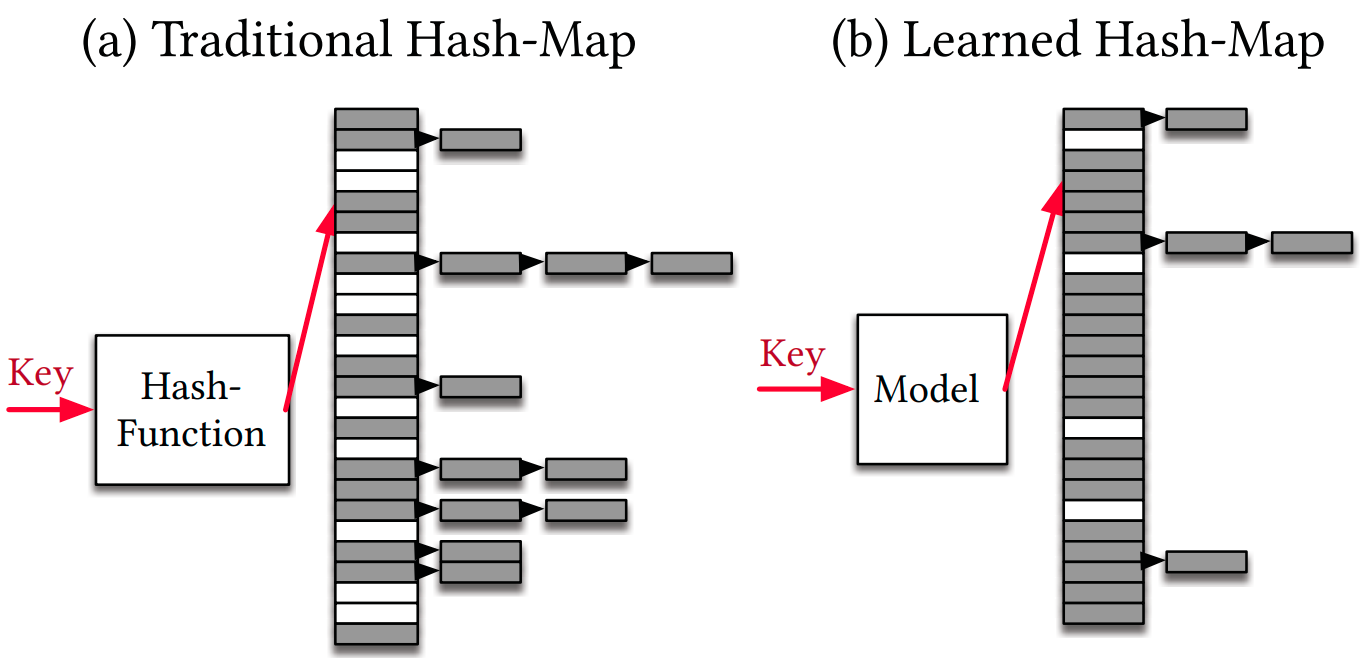
\includegraphics[scale=0.2]{figures/learned_index.png}
	\caption{Traditional Hash-map vs Learned Hash-map \cite{learning-index}}
	\label{fig:learned_index}
\end{figure}

\vspace{1mm}
\noindent

